\subsection{How2Run}
In order to successfully run, the executable of main.cpp and books.csv must be in the same directory. 
Commands that can be run are:
\begin{itemize}
\item g++ -g main.cpp
\item ./a.out
\end{itemize}
sorted\_books.csv will be created if the input file is present and thus the sorting is correct. If the sorting is wrong the output file will not be created. 
\subsection{Performance Analysis and Part2.c}

The performance analysis includes gprof for profiling and gprof2dot for the visualisations. Gprof counts how many times each function is run by putting print statements around the functions. In order to use gprof, -pg flag must be given during compile time. When the executable is run a gmon.out file is created which gprof reads and creates a flat profile and a call graph in text. Gprof2dot takes text input and creates images of call graphs with execution information. 

In the first run of my analysis, I realised that the parser was taking 50\% of the execution time. The reason for that as it can be seen at Figure \ref{malloc}, is the vector.push\_back function utilised the malloc() for vector significantly. As the input gets larger it created a growing overhead. To solve it I reserved the maximum expected size at the beginning and in the end of parsing made it shrink\_to\_fit() to not allocate more than necessary memory. 

\begin{figure}[H]
\begin{center}
\leavevmode
\includegraphics[width=350pt]{1sttry.png}
\caption{O2 optimised and compiled by g++}
\label{malloc}
\end{center}
\end{figure}


In my first iteration of the code, to see that the algorithm is working, the parsed vector was directly accessed and sorted by using string to float (stoa) function extensively. This caused an overhead as the complexity of the sorting algorithm got reflected in stoa() function as well which can be observed at Figure \ref{stoa}.
\begin{figure}[H]
\begin{center}
\leavevmode
\includegraphics[width=350pt]{output_o2optimised.png}
\caption{O2 optimised and compiled by g++}
\label{stoa}
\end{center}
\end{figure}

To remove the stoa() overhead, the reading of average rating number and the sorting of vectors must have been decoupled from the reading of the parsed vector. To achieve the decoupling two arrays of integers were considered. The unsorted\_values\[\] array included the essence of the read file. At every index i similar to row is the integer rating number. The read operation and comparison is performed on this array with the index provided from the proceeding array which holds the indices. The stof() operation is done once per row in this way in the extractor() function.
To accomodate swap operations another array, sorted\_keys\[\], holding the indices of the unsorted\_values array is created. Initially Arr\[i\] = i as they are unsorted. To perform swap, two index values residing in sorted\_keys array is swapped.  
To ensure the new index based sorting system is safe, a new class with these arrays is declared and made a global object. The class has a getValue() and swap operation. Sorting functions do not access the arrays directly. 

After making these changes the parser() function is still taking 100\% execution time as it can be seen at Figure \ref{parser}. After investigating, the problem came out to be that push\_back function had a direct argument making it do unnecessary copy operations where instead std::move would make the operation more direct. After making the changes the execution time of parser() fell into a reasonable percentage as in Figure \ref{parserfix} and Figure \ref{parserfix_clang}.  


\begin{figure}[H]
\begin{center}
\leavevmode
\includegraphics[width=0.5\textwidth]{output_o3optimised3_crop_parser.png}
\caption{O3 optimised and compiled by g++}
\label{parser}
\end{center}
\end{figure}

\begin{figure}[H]
\begin{center}
\leavevmode
\includegraphics[width=0.5\textwidth]{output_o3optimised5.png}
\caption{O3 optimised and compiled by g++}
\label{parserfix}
\end{center}
\end{figure}
\begin{figure}[H]
\begin{center}
\leavevmode
\includegraphics[width=0.5\textwidth]{output_clango3optimised6.png}
\caption{O3 optimised and compiled by clang++}
\label{parserfix_clang}
\end{center}
\end{figure}
The optimisations made by the compilers play a critical role at the performance of various parts of the code. Parser is optimised heavily in clang but not in gcc and they output different execution percentages. Apart from parser() the compiler also tries to optimize quicksort() function. In clang it is possible to view several optimizations made by the compiler on high level code with a tool named opt-viewer. In order to use it, -fsave-optimization-record -foptimization-record-file arguments should be given to clang. A yaml file containing optimisations will be generated. Opt-viewer can use the yaml file and generate html files. The opt-viewer is written in Python and it is in the llvm repository.


\begin{figure}[H]
\begin{center}
\leavevmode
\includegraphics[width=0.5\textwidth]{partition_optviewer.png}
\caption{Optimisations of Clang provided by Opt-Viewer}
\label{part_opt}
\end{center}
\end{figure}

\begin{figure}[H]
\begin{center}
\leavevmode
\includegraphics[width=0.5\textwidth]{quicksort_optviewer.png}
\caption{Optimisations of Clang provided by Opt-Viewer}
\label{qs_opt}
\end{center}
\end{figure}
The optimisations of Clang in the partition() function can be viewed at Figure \ref{part_opt} which are minimal. The optimisations on quicksort() can be seen at Figure \ref{qs_opt} which includes tail call elimination. 

The function call statistics are present in gprof but to have the statistics embedded in the code several counter variables are added and printed after the counting is finished. The time difference between entering the quicksort() is also printed. The time taken by quicksort is varying so the screenshots include 5 samples of the time difference. Similarly the screenshots for the second quicksort algorithm are given.


\begin{figure}[H]
\begin{center}
\leavevmode
\includegraphics[width=0.5\textwidth]{qsmax.png}
\caption{Duration time of quicksort execution and function counts with 100\% input }
\label{qs_max}
\end{center}
\end{figure}
\begin{figure}[H]
\begin{center}
\leavevmode
\includegraphics[width=0.5\textwidth]{qshalf.png}
\caption{Duration time of quicksort execution and function counts with 50\% input }
\label{qs_half}
\end{center}
\end{figure}
\begin{figure}[H]
\begin{center}
\leavevmode
\includegraphics[width=0.5\textwidth]{qsquarter.png}
\caption{Duration time of quicksort execution and function counts with 25\% input }
\label{qs_quarter}
\end{center}
\end{figure}
\begin{figure}[H]
\begin{center}
\leavevmode
\includegraphics[width=0.5\textwidth]{qsquarterhalf.png}
\caption{Duration time of quicksort execution and function counts with 12\% input }
\label{qs_qhalf}
\end{center}
\end{figure}

\begin{figure}[H]
\begin{center}
\leavevmode
\includegraphics[width=0.5\textwidth]{qs2max.png}
\caption{Duration time of the second quicksort execution and function counts with 100\% input }
\label{qs_max}
\end{center}
\end{figure}
\begin{figure}[H]
\begin{center}
\leavevmode
\includegraphics[width=0.5\textwidth]{qs2half.png}
\caption{Duration time of the second quicksort execution and function counts with 50\% input }
\label{qs_half}
\end{center}
\end{figure}
\begin{figure}[H]
\begin{center}
\leavevmode
\includegraphics[width=0.5\textwidth]{qs2quarter.png}
\caption{Duration time of the second quicksort execution and function counts with 25\% input }
\label{qs_quarter}
\end{center}
\end{figure}
\begin{figure}[H]
\begin{center}
\leavevmode
\includegraphics[width=0.5\textwidth]{qs2quarterhalf.png}
\caption{Duration time of the second quicksort execution and function counts with 12\% input }
\label{qs_qhalf}
\end{center}
\end{figure}
\begin{table}
\begin{center}
\begin{tabular}{|c c c c|}
 \hline
    Input Size & Average Running Time (us) & Swap Count & Partition Count\\ [0.5ex]
 \hline
    1388 & 957 & 6051 & 1158\\
    2779 & 2465 & 13393 & 2386\\
    5562 & 3768 & 24529 & 4847\\
    11126 & 8148 & 51601 & 9815 \\[1ex]
 \hline
\end{tabular}
\end{center}
    \caption{Statistics regarding execution time and function call counts of the first algorithm}
    \label{stats1}
\end{table}
\begin{table}
\begin{center}
\begin{tabular}{|c c c c|}
 \hline
    Input Size & Average Running Time (us) & Swap Count & Partition Count\\ [0.5ex]
 \hline
    1386 & 404 & 4594 & 840\\
    2777 & 1090 & 10314 & 1630\\
    5560 & 2217 & 23299 & 3270\\
    11126 & 2541 & 51948 & 6522 \\[1ex]
 \hline
\end{tabular}
\end{center}
    \caption{Statistics regarding execution time and function call counts of the second algorithm}
    \label{stats2}
\end{table}
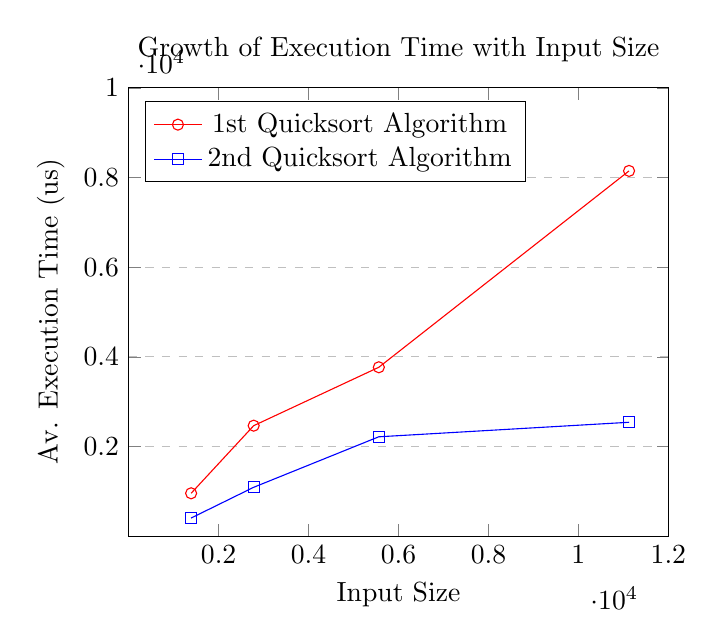
\begin{tikzpicture}
\begin{axis}[
        title={Growth of Execution Time with Input Size},
    xlabel={Input Size},
    ylabel={Av. Execution Time (us) },
    xmin=0, xmax=12000,
    ymin=0, ymax=10000,
    xtick={2000,4000,6000,8000,10000, 12000},
    ytick={2000,4000,6000,8000,10000},
    legend pos=north west,
    ymajorgrids=true,
    grid style=dashed
]
\addplot[
    color=red,
    mark=o,
    ]
    coordinates {
    (1388,957)(2779,2465)(5562,3768)(11126,8148)
    };
\addplot[
    color=blue,
    mark=square,
    ]
    coordinates {
    (1386,404)(2777,1090)(5560,2217)(11126,2541)
    };
    \legend{1st Quicksort Algorithm, 2nd Quicksort Algorithm}

\end{axis}
\end{tikzpicture}

As it can be seen at Table \ref{stats1} and \ref{stats2}, smaller input sizes cause significant reduction in execution time.

\par
\subsubsection{Efficiency and Part2.d}

I think the second algorithm is more efficient because every swap contributes to both sides of the pivot. However in the first algorithm swaps are done to move single elements rather than pairs. 

The recurrence equation for quicksort is \( T(n) = T(n_1) + T(n - 1 - n_1) + (n - 1)\). As the partition is not guaranteed to split the array into two the, \( n_1\) is given as the pivot index. 

\par

The worst case scenario is having one of the subarrays empty everytime which results the following recurrence equation\( T(n) = T(0) + T(n - 1 ) + (n - 1) = T(n - 1) + (n - 1)\). \(T(n - 1) + (n - 1) = T(n - 2) + (n - 2) + (n - 1) = \sum_{i=1}^{n-1} i  = (n - 1)n/2 \) which means the \(O(n^2)  \) is the average worst case asymptotic bound for quicksort.

The best case scenario occurs when there is no empty array and the divided arrays are of same size. For this condition, \( n_1 = (n - 1)/2 \). The resulting recurrence equation is \(T(n) = 2*T(\frac{n-1}{2} + (n - 1)) \). It is the same as merge sort \(O(n*\log n ) \).  

The average case scenario assumes uniform distribution of inputs. The pivot index \(n_1\) can be 0 to n - 1 with equal probabaility. The slides of the course state that the \(E[ number of comparisons]\) is \(O(n*\log n ) \). The number of comparisons will dominate the runtime.

\subsubsection{Worst Case Scenario and Part2.e}
If the input is already sorted, with QS1 pivot is selected as the highest index element. So the partition results with the elements less than the pivot and and an empty array. Every partition results with an array smaller by one. As the n length  array is traversed, partition runs n times. Partition includes n comparisons so the worst case runtime of \(O(n^2) \) is achieved with this input.


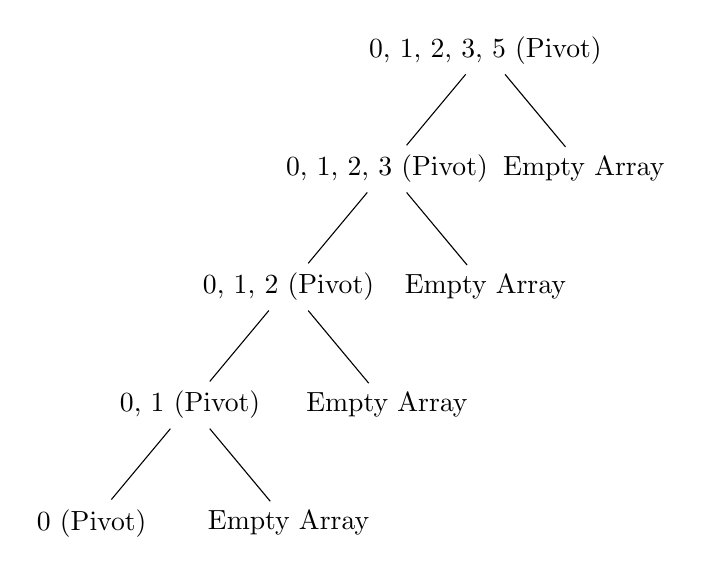
\begin{tikzpicture}
    \node {0, 1, 2, 3, 5 (Pivot)} [sibling distance = 2.5cm]
    child {node {0, 1, 2, 3 (Pivot)}
    child {node {0, 1, 2 (Pivot)}
    child {node {0, 1 (Pivot)}
    child {node {0 (Pivot)}}
    child {node {Empty Array}}}
    child {node {Empty Array}}}
    child {node {Empty Array}}}
    child {node {Empty Array}};
\end{tikzpicture}

The reason is the fixed pivot index, a random pivot could result more non-empty arrays. A checker at the beginning could help detect already sorted inputs. Also Knuth suggests using insertion sort after M sized files are produced by quicksort.
